% vim: set spell spelllang=en tw=100 et sw=4 sts=4 foldmethod=marker foldmarker={{{,}}} :

\documentclass{beamer}

\usepackage{tikz}
\usepackage{xcolor}
\usepackage{complexity}
\usepackage{hyperref}
\usepackage{microtype}
\usepackage{amsmath}                   % \operatorname
\usepackage{amsfonts}                  % \mathcal
\usepackage{amssymb}                   % \nexists
\usepackage{gnuplot-lua-tikz}          % graphs
\usepackage[vlined]{algorithm2e} % algorithms
\usepackage{centernot}

\usetikzlibrary{shapes, arrows, shadows, calc, positioning, fit}
\usetikzlibrary{decorations.pathreplacing, decorations.pathmorphing, shapes.misc}
\usetikzlibrary{tikzmark}

\definecolor{uofguniversityblue}{rgb}{0, 0.219608, 0.396078}

\definecolor{uofgheather}{rgb}{0.356863, 0.32549, 0.490196}
\definecolor{uofgaquamarine}{rgb}{0.603922, 0.72549, 0.678431}
\definecolor{uofgslate}{rgb}{0.309804, 0.34902, 0.380392}
\definecolor{uofgrose}{rgb}{0.823529, 0.470588, 0.709804}
\definecolor{uofgmocha}{rgb}{0.709804, 0.564706, 0.47451}
\definecolor{uofgsandstone}{rgb}{0.321569, 0.278431, 0.231373}
\definecolor{uofgforest}{rgb}{0, 0.2, 0.129412}
\definecolor{uofglawn}{rgb}{0.517647, 0.741176, 0}
\definecolor{uofgcobalt}{rgb}{0, 0.615686, 0.92549}
\definecolor{uofgturquoise}{rgb}{0, 0.709804, 0.819608}
\definecolor{uofgsunshine}{rgb}{1.0, 0.862745, 0.211765}
\definecolor{uofgpumpkin}{rgb}{1.0, 0.72549, 0.282353}
\definecolor{uofgthistle}{rgb}{0.584314, 0.070588, 0.447059}
\definecolor{uofgrust}{rgb}{0.603922, 0.227451, 0.023529}
\definecolor{uofgburgundy}{rgb}{0.490196, 0.133333, 0.223529}
\definecolor{uofgpillarbox}{rgb}{0.701961, 0.047059, 0}
\definecolor{uofglavendar}{rgb}{0.356863, 0.301961, 0.580392}

\tikzset{vertex/.style={draw, circle, inner sep=3pt, minimum size=0.5cm, font=\small\bfseries}}
\tikzset{notvertex/.style={vertex, color=white, text=black}}
\tikzset{plainvertex/.style={vertex}}
\tikzset{selectedvertex/.style={vertex, fill=uofgcobalt}}
\tikzset{selectedvertex2/.style={vertex, fill=uofglawn}}
\tikzset{redvertex/.style={vertex, fill=uofgpillarbox}}
\tikzset{edge/.style={color=black!50!white}}
\tikzset{bedge/.style={ultra thick}}

% {{{ theme things
\useoutertheme[footline=authortitle]{miniframes}
\useinnertheme{rectangles}

\setbeamerfont{block title}{size={}}
\setbeamerfont{title}{size=\large,series=\bfseries}
\setbeamerfont{section title}{size=\large,series=\mdseries}
\setbeamerfont{author}{size=\normalsize,series=\mdseries}
\setbeamercolor*{structure}{fg=uofguniversityblue}
\setbeamercolor*{palette primary}{use=structure,fg=black,bg=white}
\setbeamercolor*{palette secondary}{use=structure,fg=white,bg=uofgcobalt}
\setbeamercolor*{palette tertiary}{use=structure,fg=white,bg=uofguniversityblue}
\setbeamercolor*{palette quaternary}{fg=white,bg=black}

\setbeamercolor*{titlelike}{parent=palette primary}

\beamertemplatenavigationsymbolsempty

\setbeamertemplate{title page}
{
    \begin{tikzpicture}[remember picture, overlay]
        \node at (current page.north west) {
            \begin{tikzpicture}[remember picture, overlay]
                \fill [fill=uofguniversityblue, anchor=north west] (0, 0) rectangle (\paperwidth, -2.6cm);
            \end{tikzpicture}
        };

        \node (logo) [anchor=north east, shift={(-0.6cm,-0.6cm)}] at (current page.north east) {
            \includegraphics*[keepaspectratio=true,scale=0.7]{UoG_keyline.pdf}
        };

        \node [anchor=west, xshift=0.2cm] at (current page.west |- logo.west) {
            \begin{minipage}{0.65\paperwidth}\raggedright
                {\usebeamerfont{title}\usebeamercolor[white]{}\inserttitle}\\[0.1cm]
                {\usebeamerfont{author}\usebeamercolor[white]{}\insertauthor}
            \end{minipage}
        };
    \end{tikzpicture}
}

\setbeamertemplate{section page}
{
    \begin{centering}
        \begin{beamercolorbox}[sep=12pt,center]{part title}
            \usebeamerfont{section title}\insertsection\par
        \end{beamercolorbox}
    \end{centering}
}

\newcommand{\frameofframes}{/}
\newcommand{\setframeofframes}[1]{\renewcommand{\frameofframes}{#1}}

\makeatletter
\setbeamertemplate{footline}
{%
    \begin{beamercolorbox}[colsep=1.5pt]{upper separation line foot}
    \end{beamercolorbox}
    \begin{beamercolorbox}[ht=2.5ex,dp=1.125ex,%
        leftskip=.3cm,rightskip=.3cm plus1fil]{author in head/foot}%
        \leavevmode{\usebeamerfont{author in head/foot}\insertshortauthor}%
        \hfill%
        {\usebeamerfont{institute in head/foot}\usebeamercolor[fg]{institute in head/foot}\insertshortinstitute}%
    \end{beamercolorbox}%
    \begin{beamercolorbox}[ht=2.5ex,dp=1.125ex,%
        leftskip=.3cm,rightskip=.3cm plus1fil]{title in head/foot}%
        {\usebeamerfont{title in head/foot}\insertshorttitle}%
        \hfill%
        {\usebeamerfont{frame number}\usebeamercolor[fg]{frame number}\insertframenumber~\frameofframes~\inserttotalframenumber}
    \end{beamercolorbox}%
    \begin{beamercolorbox}[colsep=1.5pt]{lower separation line foot}
    \end{beamercolorbox}
}

\makeatletter
\newenvironment{nearlyplainframe}[2][]{
    \def\beamer@entrycode{\vspace*{-\headheight}}
    \setbeamertemplate{headline}
    {%
        \begin{beamercolorbox}[colsep=1.5pt]{upper separation line head}
        \end{beamercolorbox}
        \begin{beamercolorbox}[ht=0.5ex,dp=0.125ex,%
            leftskip=.3cm,rightskip=.3cm plus1fil]{title in head/foot}%
        \end{beamercolorbox}%
        \begin{beamercolorbox}[ht=0.5ex,dp=0.125ex,%
            leftskip=.3cm,rightskip=.3cm plus1fil]{author in head/foot}%
        \end{beamercolorbox}%
        \begin{beamercolorbox}[colsep=1.5pt]{lower separation line head}
        \end{beamercolorbox}
        \vspace*{\headheight}
    }

    \setbeamertemplate{footline}
    {%
        \begin{beamercolorbox}[colsep=1.5pt]{upper separation line foot}
        \end{beamercolorbox}
        \begin{beamercolorbox}[ht=0.5ex,dp=0.125ex,%
            leftskip=.3cm,rightskip=.3cm plus1fil]{author in head/foot}%
        \end{beamercolorbox}%
        \begin{beamercolorbox}[ht=0.5ex,dp=0.125ex,%
            leftskip=.3cm,rightskip=.3cm plus1fil]{title in head/foot}%
        \end{beamercolorbox}%
        \begin{beamercolorbox}[colsep=1.5pt]{lower separation line foot}
        \end{beamercolorbox}
    }

    \begin{frame}[#1]{#2}
    }{
    \end{frame}
}
\makeatother

% }}}

\title[Finding Maximum $k$-Cliques Faster Using Lazy Global Domination]{Finding Maximum $k$-Cliques
Faster \\ Using Lazy Global Domination}
\author[Ciaran McCreesh and Patrick Prosser]{\textbf{Ciaran McCreesh} and Patrick
Prosser}

\begin{document}

{
    \usebackgroundtemplate{
        \tikz[overlay, remember picture]
        \node[at=(current page.south), anchor=south, inner sep=0pt]{\includegraphics*[keepaspectratio=true, width=\paperwidth]{background.jpg}};
    }
    \begin{frame}[plain,noframenumbering]
        \titlepage
    \end{frame}
}

\begin{frame}{Maximum Clique}
    \centering
    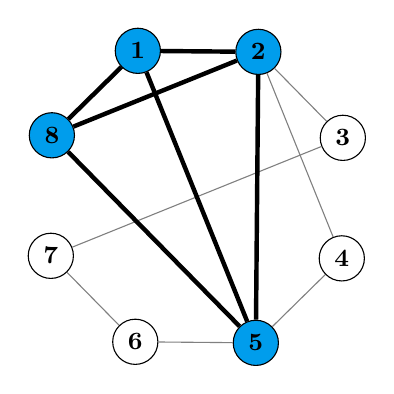
\begin{tikzpicture}
        \newcount \c
        \foreach \n in {1, ..., 8}{
            \c=\n \advance\c by -1 \multiply\c by -360 \divide\c by 8 \advance\c by 90 \advance\c by 22.5
            \ifthenelse{\n = 1 \OR \n = 2 \OR \n = 5 \OR \n = 8}{
                \node[selectedvertex] (N\n) at (\the\c:2) {\n};
            }{
                \node[plainvertex] (N\n) at (\the\c:2) {\n};
            }
        }

        \draw [edge] (N2) -- (N3);
        \draw [edge] (N2) -- (N4);
        \draw [edge] (N3) -- (N7);
        \draw [edge] (N4) -- (N5);
        \draw [edge] (N5) -- (N6);
        \draw [edge] (N6) -- (N7);

        \draw [bedge] (N1) -- (N2);
        \draw [bedge] (N1) -- (N5);
        \draw [bedge] (N1) -- (N8);
        \draw [bedge] (N2) -- (N5);
        \draw [bedge] (N2) -- (N8);
        \draw [bedge] (N5) -- (N8);
    \end{tikzpicture}
\end{frame}

\begin{frame}{Maximum $k$-Clique}
    \centering
    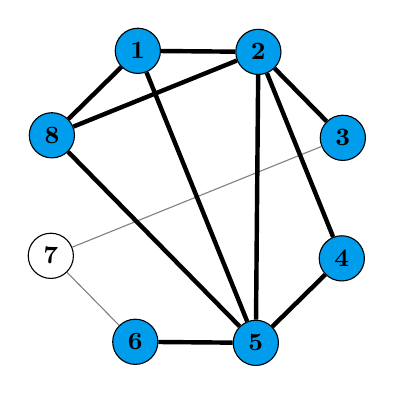
\begin{tikzpicture}
        \newcount \c
        \foreach \n in {1, ..., 8}{
            \c=\n \advance\c by -1 \multiply\c by -360 \divide\c by 8 \advance\c by 90 \advance\c by 22.5
            \ifthenelse{\n = 1 \OR \n = 2 \OR \n = 3 \OR \n = 4 \OR \n = 5 \OR \n = 6 \OR \n = 8}{
                \node[selectedvertex] (N\n) at (\the\c:2) {\n};
            }{
                \node[plainvertex] (N\n) at (\the\c:2) {\n};
            }
        }

        \draw [edge] (N3) -- (N7);
        \draw [edge] (N6) -- (N7);

        \draw [bedge] (N1) -- (N2);
        \draw [bedge] (N1) -- (N5);
        \draw [bedge] (N1) -- (N8);
        \draw [bedge] (N2) -- (N5);
        \draw [bedge] (N2) -- (N8);
        \draw [bedge] (N5) -- (N8);
        \draw [bedge] (N2) -- (N3);
        \draw [bedge] (N2) -- (N4);
        \draw [bedge] (N4) -- (N5);
        \draw [bedge] (N5) -- (N6);
    \end{tikzpicture}
\end{frame}

\begin{frame}{Maximum $k$-Club}
    \centering
    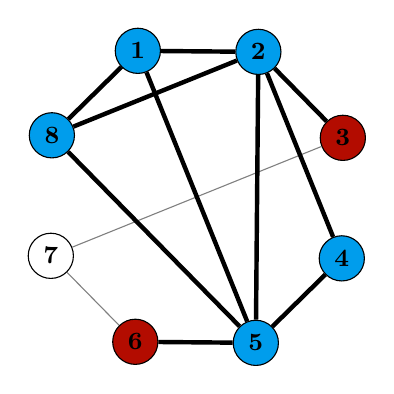
\begin{tikzpicture}
        \newcount \c
        \foreach \n in {1, ..., 8}{
            \c=\n \advance\c by -1 \multiply\c by -360 \divide\c by 8 \advance\c by 90 \advance\c by 22.5
            \ifthenelse{\n = 1 \OR \n = 2 \OR \n = 4 \OR \n = 5 \OR \n = 8}{
                \node[selectedvertex] (N\n) at (\the\c:2) {\n};
            }{
                \ifthenelse{\n = 3 \OR \n = 6}{
                    \node[redvertex] (N\n) at (\the\c:2) {\n};
                }{
                    \node[plainvertex] (N\n) at (\the\c:2) {\n};
                }
            }
        }

        \draw [edge] (N3) -- (N7);
        \draw [edge] (N6) -- (N7);

        \draw [bedge] (N1) -- (N2);
        \draw [bedge] (N1) -- (N5);
        \draw [bedge] (N1) -- (N8);
        \draw [bedge] (N2) -- (N5);
        \draw [bedge] (N2) -- (N8);
        \draw [bedge] (N5) -- (N8);
        \draw [bedge] (N2) -- (N3);
        \draw [bedge] (N2) -- (N4);
        \draw [bedge] (N4) -- (N5);
        \draw [bedge] (N5) -- (N6);
    \end{tikzpicture}
\end{frame}

\begin{frame}{Existing Work}
    \begin{itemize}
        \item Many computational papers on the $k$-club problem.
            \begin{itemize}
                \item Not a hereditary property, and modelling it is hard, so lots of scope for
                    being clever.
            \end{itemize}

        \item ``Unlike the maximum clique problem, the maximum $k$-clique problem has not been the
            subject of extensive research and we are not aware of any computational results for this
            problem to date.'' (Shahinpour and Butenko, 2013)
    \end{itemize}
\end{frame}

\begin{frame}{Reducing $k$-Clique to Clique}
    \centering
    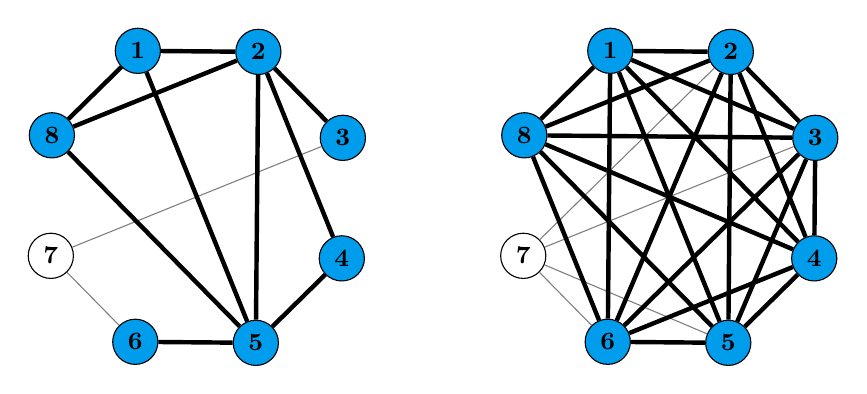
\begin{tikzpicture}
        \begin{scope}
            \newcount \c
            \foreach \n in {1, ..., 8}{
                \c=\n \advance\c by -1 \multiply\c by -360 \divide\c by 8 \advance\c by 90 \advance\c by 22.5
                \ifthenelse{\n = 1 \OR \n = 2 \OR \n = 3 \OR \n = 4 \OR \n = 5 \OR \n = 6 \OR \n = 8}{
                    \node[selectedvertex] (N\n) at (\the\c:2) {\n};
                }{
                    \node[plainvertex] (N\n) at (\the\c:2) {\n};
                }
            }

            \draw [edge] (N3) -- (N7);
            \draw [edge] (N6) -- (N7);

            \draw [bedge] (N1) -- (N2);
            \draw [bedge] (N1) -- (N5);
            \draw [bedge] (N1) -- (N8);
            \draw [bedge] (N2) -- (N5);
            \draw [bedge] (N2) -- (N8);
            \draw [bedge] (N5) -- (N8);
            \draw [bedge] (N2) -- (N3);
            \draw [bedge] (N2) -- (N4);
            \draw [bedge] (N4) -- (N5);
            \draw [bedge] (N5) -- (N6);
        \end{scope}
        \begin{scope}[xshift=6cm]
            \newcount \c
            \foreach \n in {1, ..., 8}{
                \c=\n \advance\c by -1 \multiply\c by -360 \divide\c by 8 \advance\c by 90 \advance\c by 22.5
                \ifthenelse{\n = 1 \OR \n = 2 \OR \n = 3 \OR \n = 4 \OR \n = 5 \OR \n = 6 \OR \n = 8}{
                    \node[selectedvertex] (N\n) at (\the\c:2) {\n};
                }{
                    \node[plainvertex] (N\n) at (\the\c:2) {\n};
                }
            }

            \draw [edge] (N2) -- (N7);
            \draw [edge] (N3) -- (N7);
            \draw [edge] (N5) -- (N7);
            \draw [edge] (N6) -- (N7);

            \draw [bedge] (N1) -- (N2);
            \draw [bedge] (N1) -- (N3);
            \draw [bedge] (N1) -- (N4);
            \draw [bedge] (N1) -- (N5);
            \draw [bedge] (N1) -- (N6);
            \draw [bedge] (N1) -- (N8);
            \draw [bedge] (N2) -- (N3);
            \draw [bedge] (N2) -- (N4);
            \draw [bedge] (N2) -- (N5);
            \draw [bedge] (N2) -- (N6);
            \draw [bedge] (N2) -- (N8);
            \draw [bedge] (N3) -- (N4);
            \draw [bedge] (N3) -- (N5);
            \draw [bedge] (N3) -- (N6);
            \draw [bedge] (N3) -- (N8);
            \draw [bedge] (N4) -- (N5);
            \draw [bedge] (N4) -- (N6);
            \draw [bedge] (N4) -- (N8);
            \draw [bedge] (N5) -- (N6);
            \draw [bedge] (N5) -- (N8);
            \draw [bedge] (N6) -- (N8);
        \end{scope}
    \end{tikzpicture}
\end{frame}

\begin{frame}{But Is This Practical?}
    \begin{itemize}
        \item We probably want to work with large sparse graphs as inputs.
        \item There are many good maximum clique algorithms for large sparse graphs.
        \item But $G^k$ is large and dense!
        \item There are also good maximum clique algorithms for small dense graphs, but small dense
            graphs can be \emph{very} hard.
            \begin{itemize}
                \item $\omega(\operatorname{G}(500, 0.9))$ can't be solved in a CPU-decade.
            \end{itemize}
    \end{itemize}
\end{frame}

\begin{frame}{The Good News}
    \begin{itemize}
        \item Start with a state-of-the-art maximum clique algorithm for small dense graphs.
        \item Replace cubic preprocessing and inference with cheaper quadratic algorithms.
        \item Spend some time making sure the $G^k$ reduction fast.
        \item Buy a hefty amount of RAM.
    \end{itemize}
\end{frame}

\begin{frame}{The Results ($k \in \{2, 3, 4\}$)}
    \begin{itemize}
        \item Erd\H{o}s collaboration graphs:
            \begin{itemize}
                \item $|V| \le 6,927$, $|E| \le 11,850$, $D(G^k) \le 0.57$ (or $= 1$).
                \item 16 take $<1s$, 2 take $<12s$, 3 $>1h$.
            \end{itemize}

        \item DIMACS 2 Clique Graphs with diameter $> 2$:
            \begin{itemize}
                \item $|V| \le 500$, $|E| \le 46,627$, $D(G^k) \le 0.87$ (or $= 1$)
                \item 22 take $<1s$, 2 take $>1h$.
            \end{itemize}

        \item DIMACS 10 Partitioning Graphs (smallest 20):
            \begin{itemize}
                \item $|V| \le 36,519$, $|E| \le 1,007,284$, $D(G^k) \le 0.67$.
                \item 2 take $>1h$, most take well under a minute.
            \end{itemize}

        \item DIMACS 10 Clustering Graphs (smallest 20):
            \begin{itemize}
                \item $|V| \le 40,421$, $|E| \le 175,691$, $D(G^k) \le 0.99$.
                \item 7 take $>1h$, most take well under a minute.
            \end{itemize}
    \end{itemize}
\end{frame}

\begin{frame}{But We Can Do Better}
    \centering
    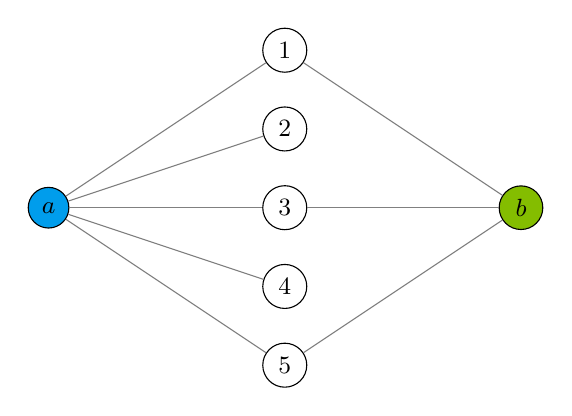
\begin{tikzpicture}
        \begin{scope}
            \node[selectedvertex] (Na) at (0, 2) {$a$};
            \node[selectedvertex2] (Nb) at (6, 2) {$b$};

            \node[plainvertex] (N1) at (3, 4) {$1$};
            \node[plainvertex] (N2) at (3, 3) {$2$};
            \node[plainvertex] (N3) at (3, 2) {$3$};
            \node[plainvertex] (N4) at (3, 1) {$4$};
            \node[plainvertex] (N5) at (3, 0) {$5$};

            \draw [edge] (Na) -- (N1);
            \draw [edge] (Na) -- (N2);
            \draw [edge] (Na) -- (N3);
            \draw [edge] (Na) -- (N4);
            \draw [edge] (Na) -- (N5);

            \draw [edge] (Nb) -- (N1);
            \draw [edge] (Nb) -- (N3);
            \draw [edge] (Nb) -- (N5);
        \end{scope}
    \end{tikzpicture}
\end{frame}

\begin{frame}{Better Results!}
    \begin{itemize}
        \item Erd\H{o}s collaboration graphs:
            \begin{itemize}
                \item The three open instances now take 3.8s, 69.4s, 207.3s.
            \end{itemize}

        \item DIMACS 2 Clique Graphs:
            \begin{itemize}
                \item The two open instances now take 0.1s.
            \end{itemize}

        \item DIMACS 10 Partitioning Graphs:
            \begin{itemize}
                \item One open instance now takes 16.9s, the other still takes $>1h$.
            \end{itemize}

        \item DIMACS 10 Clustering Graphs:
            \begin{itemize}
                \item Two open instances closed.
            \end{itemize}

        \item Not a universal success, though:
            \begin{itemize}
                \item Factor of 10 slowdown on a few fairly easy instances.
                \item Without laziness, the results are terrible\ldots
            \end{itemize}
    \end{itemize}
\end{frame}

\begin{frame}{What About Parallel Search?}

    \begin{itemize}
        \item Active research topic for maximum clique.
            \begin{itemize}
                \item Work stealing strategies really make a huge difference (often more so than
                    load balance)!
                \item Use parallelism to steal early, where value ordering heuristics are
                    weakest---a bit like discrepancy search or restarts.
            \end{itemize}
    \end{itemize}
\end{frame}

\begin{frame}{Even Betterer Results!}
    \begin{itemize}
        \item Two open instances closed.
        \item Improved bounds on four remaining instances.
        \item Also super-linear speedups in (at least) two cases.
        \item But only if we get it right:
            \begin{itemize}
                \item Again, work stealing strategies matter.
                \item Load balancing is harder: must use a much deeper splitting limit than for
                    typical maximum clique graphs.
            \end{itemize}
    \end{itemize}
\end{frame}

\begin{frame}{What About Random Graphs?}
    \centering
    \input{gen-graph-nodes}
\end{frame}

\begin{frame}{Conclusion}

    \begin{itemize}
        \item There are many clique relaxations (density-based, degree-based, distance-based,
            \ldots). It's often not clear which you'd want in practice.
        \item $k$-Clique tends to be easy to calculate, at least.
        \item Usually the $k$-Clique and $k$-Club numbers are the same, too.
        \item The domination rule is probably useful in other settings.
        \item Work-stealing strategies matter when doing parallel search.
    \end{itemize}
\end{frame}

\begin{frame}[plain,noframenumbering]
    \begin{center}
        \vspace*{4em}
        \url{http://www.dcs.gla.ac.uk/~ciaran} \\
        \vspace{1em}
        \href{mailto:c.mccreesh.1@research.gla.ac.uk}{\nolinkurl{c.mccreesh.1@research.gla.ac.uk}} \\
    \end{center}

    \begin{tikzpicture}[remember picture, overlay]
        \node at (current page.north west) {
            \begin{tikzpicture}[remember picture, overlay]
                \fill [fill=uofguniversityblue, anchor=north west] (0, 0) rectangle (\paperwidth, -2.6cm);
            \end{tikzpicture}
        };

        \node (logo) [anchor=north east, shift={(-0.6cm,-0.6cm)}] at (current page.north east) {
            \includegraphics*[keepaspectratio=true,scale=0.7]{UoG_keyline.pdf}
        };
    \end{tikzpicture}
\end{frame}

\end{document}


